



\tikzset{every picture/.style={line width=0.75pt}} %set default line width to 0.75pt        

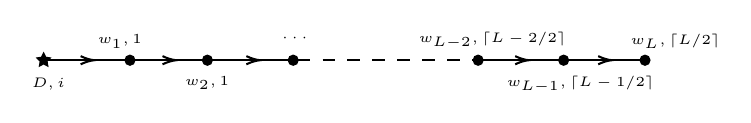
\begin{tikzpicture}[x=0.75pt,y=0.75pt,yscale=-1,xscale=1]
%uncomment if require: \path (0,149); %set diagram left start at 0, and has height of 149

%Straight Lines [id:da816633836761552] 
\draw    (226.1,47.5) -- (267.7,47.5) ;
\draw [shift={(250.5,47.5)}, rotate = 180] [color={rgb, 255:red, 0; green, 0; blue, 0 }  ][line width=0.75]    (6.56,-1.97) .. controls (4.17,-0.84) and (1.99,-0.18) .. (0,0) .. controls (1.99,0.18) and (4.17,0.84) .. (6.56,1.97)   ;
%Straight Lines [id:da6715871239500288] 
\draw    (267.7,47.5) -- (306.9,47.5) ;
\draw [shift={(290.9,47.5)}, rotate = 180] [color={rgb, 255:red, 0; green, 0; blue, 0 }  ][line width=0.75]    (6.56,-1.97) .. controls (4.17,-0.84) and (1.99,-0.18) .. (0,0) .. controls (1.99,0.18) and (4.17,0.84) .. (6.56,1.97)   ;
%Straight Lines [id:da8114254440797811] 
\draw  [dash pattern={on 4.5pt off 4.5pt}]  (309.05,47.5) -- (396,47.5) ;
%Shape: Ellipse [id:dp2602250925627204] 
\draw  [color={rgb, 255:red, 0; green, 0; blue, 0 }  ,draw opacity=1 ][fill={rgb, 255:red, 0; green, 0; blue, 0 }  ,fill opacity=1 ] (263.41,47.5) .. controls (263.41,46.29) and (264.37,45.31) .. (265.55,45.31) .. controls (266.74,45.31) and (267.7,46.29) .. (267.7,47.5) .. controls (267.7,48.71) and (266.74,49.69) .. (265.55,49.69) .. controls (264.37,49.69) and (263.41,48.71) .. (263.41,47.5) -- cycle ;
%Shape: Ellipse [id:dp480354117778226] 
\draw  [color={rgb, 255:red, 0; green, 0; blue, 0 }  ,draw opacity=1 ][fill={rgb, 255:red, 0; green, 0; blue, 0 }  ,fill opacity=1 ] (226.1,47.5) .. controls (226.1,46.29) and (227.06,45.31) .. (228.25,45.31) .. controls (229.43,45.31) and (230.39,46.29) .. (230.39,47.5) .. controls (230.39,48.71) and (229.43,49.69) .. (228.25,49.69) .. controls (227.06,49.69) and (226.1,48.71) .. (226.1,47.5) -- cycle ;
%Shape: Ellipse [id:dp7963501305169378] 
\draw  [color={rgb, 255:red, 0; green, 0; blue, 0 }  ,draw opacity=1 ][fill={rgb, 255:red, 0; green, 0; blue, 0 }  ,fill opacity=1 ] (304.75,47.5) .. controls (304.75,46.29) and (305.71,45.31) .. (306.9,45.31) .. controls (308.09,45.31) and (309.05,46.29) .. (309.05,47.5) .. controls (309.05,48.71) and (308.09,49.69) .. (306.9,49.69) .. controls (305.71,49.69) and (304.75,48.71) .. (304.75,47.5) -- cycle ;
%Straight Lines [id:da9333387423167766] 
\draw    (396,47.5) -- (437.6,47.5) ;
\draw [shift={(420.4,47.5)}, rotate = 180] [color={rgb, 255:red, 0; green, 0; blue, 0 }  ][line width=0.75]    (6.56,-1.97) .. controls (4.17,-0.84) and (1.99,-0.18) .. (0,0) .. controls (1.99,0.18) and (4.17,0.84) .. (6.56,1.97)   ;
%Straight Lines [id:da00536917711016649] 
\draw    (437.2,47.5) -- (476.4,47.5) ;
\draw [shift={(460.4,47.5)}, rotate = 180] [color={rgb, 255:red, 0; green, 0; blue, 0 }  ][line width=0.75]    (6.56,-1.97) .. controls (4.17,-0.84) and (1.99,-0.18) .. (0,0) .. controls (1.99,0.18) and (4.17,0.84) .. (6.56,1.97)   ;
%Shape: Ellipse [id:dp7159425745452884] 
\draw  [color={rgb, 255:red, 0; green, 0; blue, 0 }  ,draw opacity=1 ][fill={rgb, 255:red, 0; green, 0; blue, 0 }  ,fill opacity=1 ] (435.05,47.5) .. controls (435.05,46.29) and (436.01,45.31) .. (437.2,45.31) .. controls (438.39,45.31) and (439.35,46.29) .. (439.35,47.5) .. controls (439.35,48.71) and (438.39,49.69) .. (437.2,49.69) .. controls (436.01,49.69) and (435.05,48.71) .. (435.05,47.5) -- cycle ;
%Shape: Ellipse [id:dp1619386551141868] 
\draw  [color={rgb, 255:red, 0; green, 0; blue, 0 }  ,draw opacity=1 ][fill={rgb, 255:red, 0; green, 0; blue, 0 }  ,fill opacity=1 ] (393.85,47.5) .. controls (393.85,46.29) and (394.81,45.31) .. (396,45.31) .. controls (397.19,45.31) and (398.15,46.29) .. (398.15,47.5) .. controls (398.15,48.71) and (397.19,49.69) .. (396,49.69) .. controls (394.81,49.69) and (393.85,48.71) .. (393.85,47.5) -- cycle ;
%Shape: Ellipse [id:dp14958987046467243] 
\draw  [color={rgb, 255:red, 0; green, 0; blue, 0 }  ,draw opacity=1 ][fill={rgb, 255:red, 0; green, 0; blue, 0 }  ,fill opacity=1 ] (474.25,47.5) .. controls (474.25,46.29) and (475.21,45.31) .. (476.4,45.31) .. controls (477.59,45.31) and (478.55,46.29) .. (478.55,47.5) .. controls (478.55,48.71) and (477.59,49.69) .. (476.4,49.69) .. controls (475.21,49.69) and (474.25,48.71) .. (474.25,47.5) -- cycle ;

%Straight Lines [id:da865454873713147] 
\draw    (186.65,47.5) -- (228.25,47.5) ;
\draw [shift={(211.05,47.5)}, rotate = 180] [color={rgb, 255:red, 0; green, 0; blue, 0 }  ][line width=0.75]    (6.56,-1.97) .. controls (4.17,-0.84) and (1.99,-0.18) .. (0,0) .. controls (1.99,0.18) and (4.17,0.84) .. (6.56,1.97)   ;

%Shape: Star [id:dp35471832737069087] 
\draw  [fill={rgb, 255:red, 0; green, 0; blue, 0 }  ,fill opacity=1 ] (186.65,44.48) -- (187.52,46.28) -- (189.46,46.57) -- (188.05,47.97) -- (188.38,49.94) -- (186.65,49.01) -- (184.91,49.94) -- (185.24,47.97) -- (183.83,46.57) -- (185.78,46.28) -- cycle ;

% Text Node
\draw (211.33,33.86) node [anchor=north west][inner sep=0.75pt]  [font=\tiny]  {$w_{1} ,1 $};
% Text Node
\draw (253.33,53.86) node [anchor=north west][inner sep=0.75pt]  [font=\tiny]  {$w_{2} ,1 $};
% Text Node
\draw (300,33.86) node [anchor=north west][inner sep=0.75pt]  [font=\tiny]  {$\cdots $};
% Text Node
\draw (408.33,53.52) node [anchor=north west][inner sep=0.75pt]  [font=\tiny]  {$w_{L-1} ,\lceil L-1/2\rceil$};
% Text Node
\draw (468,33.19) node [anchor=north west][inner sep=0.75pt]  [font=\tiny]  {$w_{L} ,\lceil L/2\rceil$};
% Text Node
\draw (365.93,32.32) node [anchor=north west][inner sep=0.75pt]  [font=\tiny]  {$w_{L-2} ,\lceil L-2/2\rceil$};
% Text Node
\draw (179.47,54.37) node [anchor=north west][inner sep=0.75pt]  [font=\tiny]  {$D,i$};


\end{tikzpicture}